\chapter{NDN背景}

Named Data Network,简称NDN,是未来因特网架构的一部分。
该项目项目旨在开发一个新的互联网架构,可以对互联网目前的基于主机的,点至点的通信体系结构的和地址的弱点进行优化。
该项目研究并加以解决以下问题,以验证NDN作为未来互联网体系结构的技术挑战:
路由的可扩展性,快进,信任模型,网络安全,内容保护和隐私,以及基本的传播理论。
该NDN项目已于2010年9月资助的美国国家科学基金会NSF下的未来互联网体系结构项目的四个项目之一。
不同于现有的IP网络,NDN中不使用端到端的解决方案。

\begin{figure}
\centering
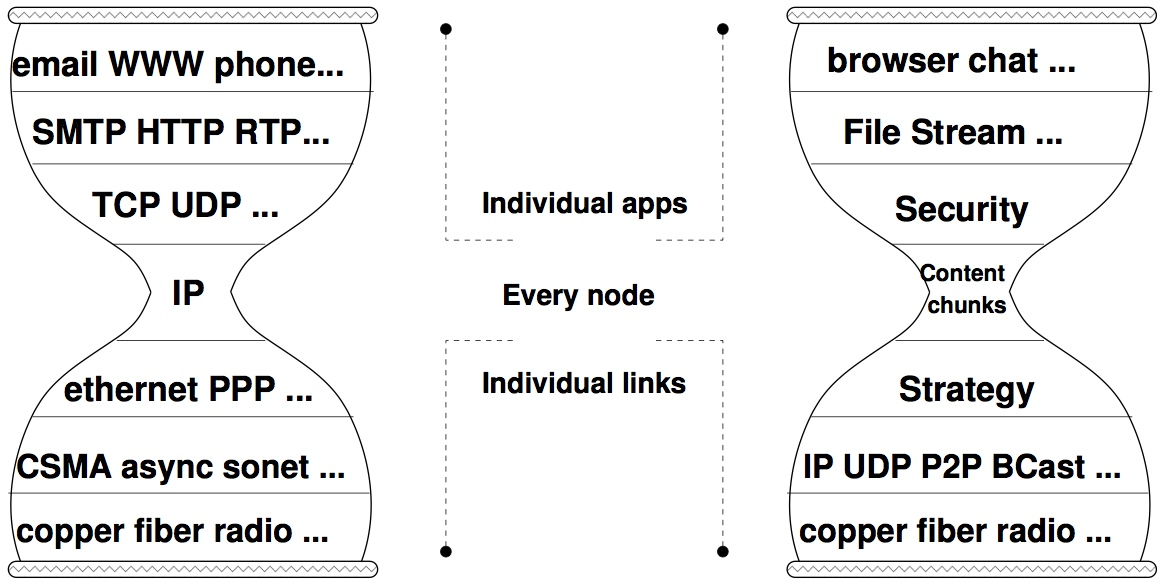
\includegraphics[width=4.5in]{png/ndn_and_ip.jpg}
\caption{NDN和IP的架构比较}
\label{}
\end{figure}

\begin{figure}[]
\centering
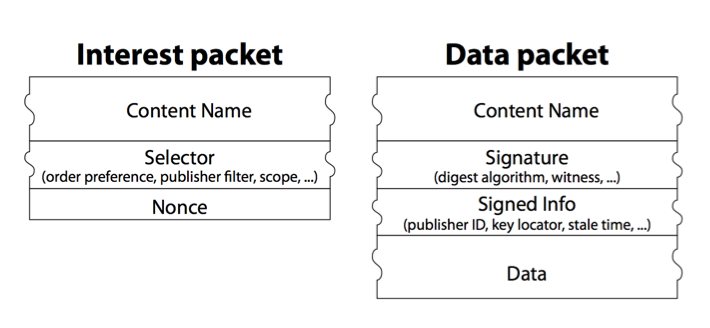
\includegraphics[width=4.5in]{png/ndn_packet.png}
\caption{NDN中得Interest和Data数据包}
\label{}
\end{figure}

在NDN通信接收端,数据数据是由消费者驱动的。
接收数据时,消费者发出一个兴趣分组,它带有用于识别所需要的数据的名称。
例如,消费者可以请求`/ustc/video/a.mpg'。
路由器记得该请求进入的端口,然后在其转发的转发兴趣报列表(FIB )中查找名称。
它是通过填充一个基于名字的路由协议。
当兴趣包达到具有所请求的数据的节点时,一个数据包被发送回,
它带有两个名称和内容数据,与生产者的签名一起。
此数据包沿着兴趣分组的反向的路径,回到消费者。
需要注意的是,无论是兴趣包还是数据包,都不携带任何主机或接口地址(如IP地址)。
兴趣包路由到数据是基于兴趣包所包含的报文的名字,数据包产生者根据由兴趣包在每个路由器跳状态信息原路返回。
NDN路由器保持兴趣包和数据一段时间,作为缓存。

\begin{figure}
\centering
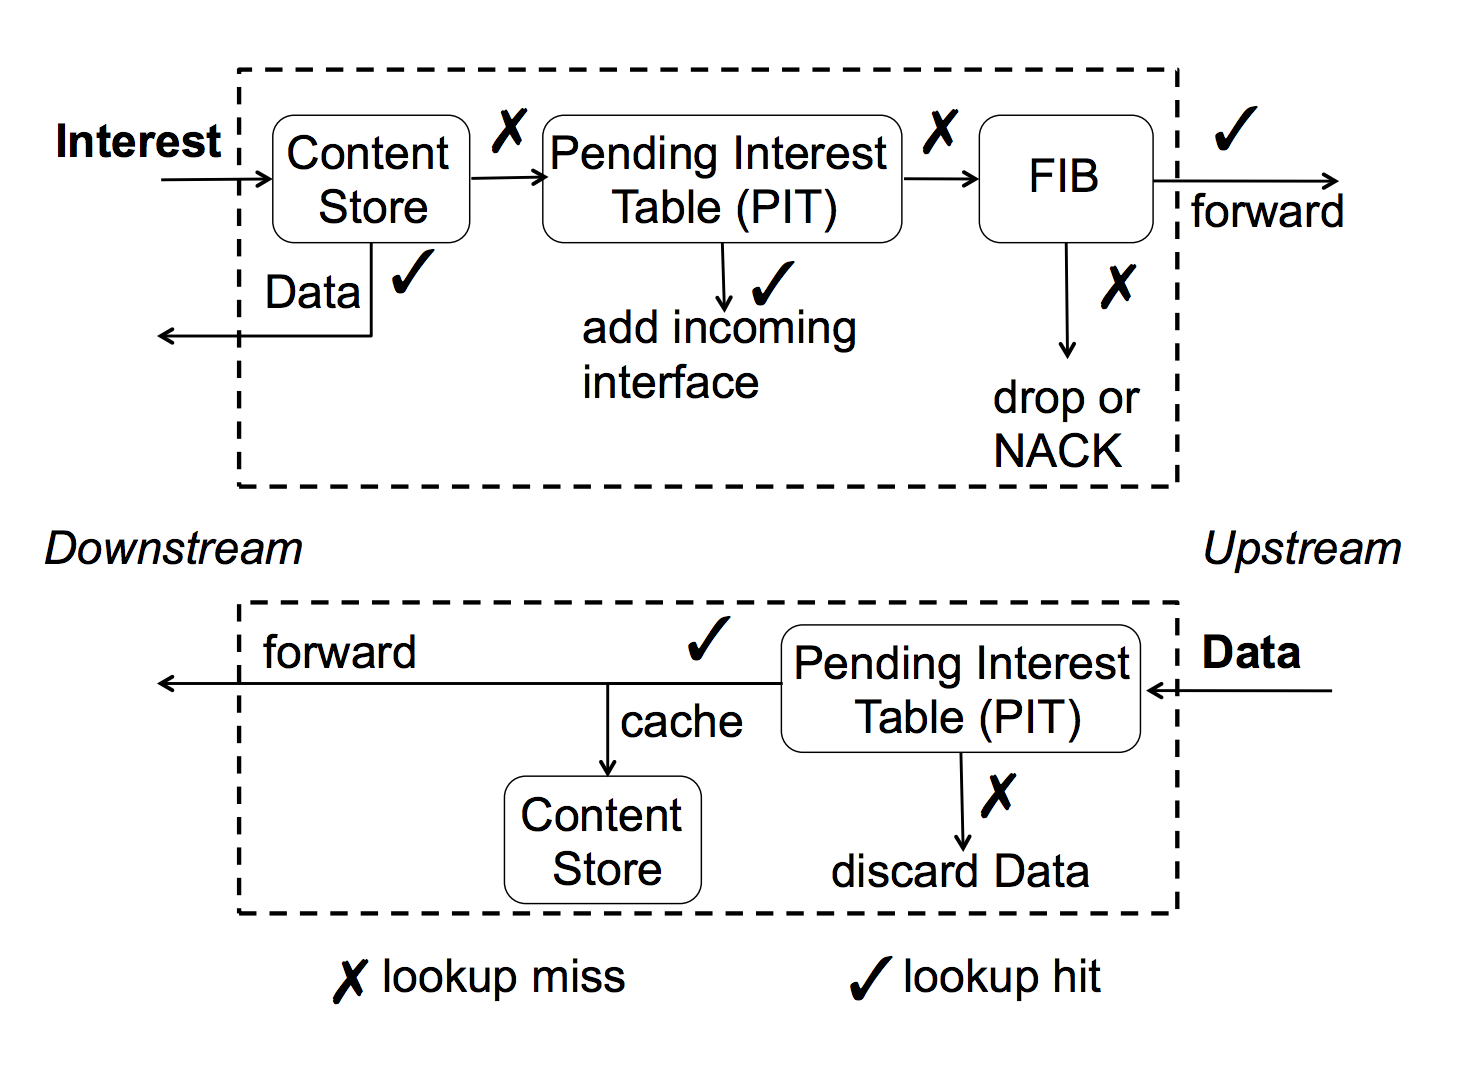
\includegraphics[width=4.5in]{png/interest_data_process.png}
\caption{NDN中处理Interest和Data数据包的流程}
\label{mobility_pic}
\end{figure}

当多个相同兴趣包所请求的为同一个数据,那么只有第一个对数据源的兴趣包会向上游发送。
该路由器然后将这个转发信息存储在转发兴趣包表( PIT )中 ,
其中每个条目包含兴趣包名和一组从接口,这些接口都是发送该兴趣包来的接口。
当数据包到达时,路由器就会找到与之对应的PIT项和数据转发到所有列出的接口PIT的条目。
路由器然后删除相应的PIT表项,并将其缓存在自己的本地缓存中。
这使用路由器的缓冲存储器,并采用高速缓存替换策略。
数据有请求它的兴趣包的精确相同的路径,但是传输方向相反。

\begin{figure}
\centering
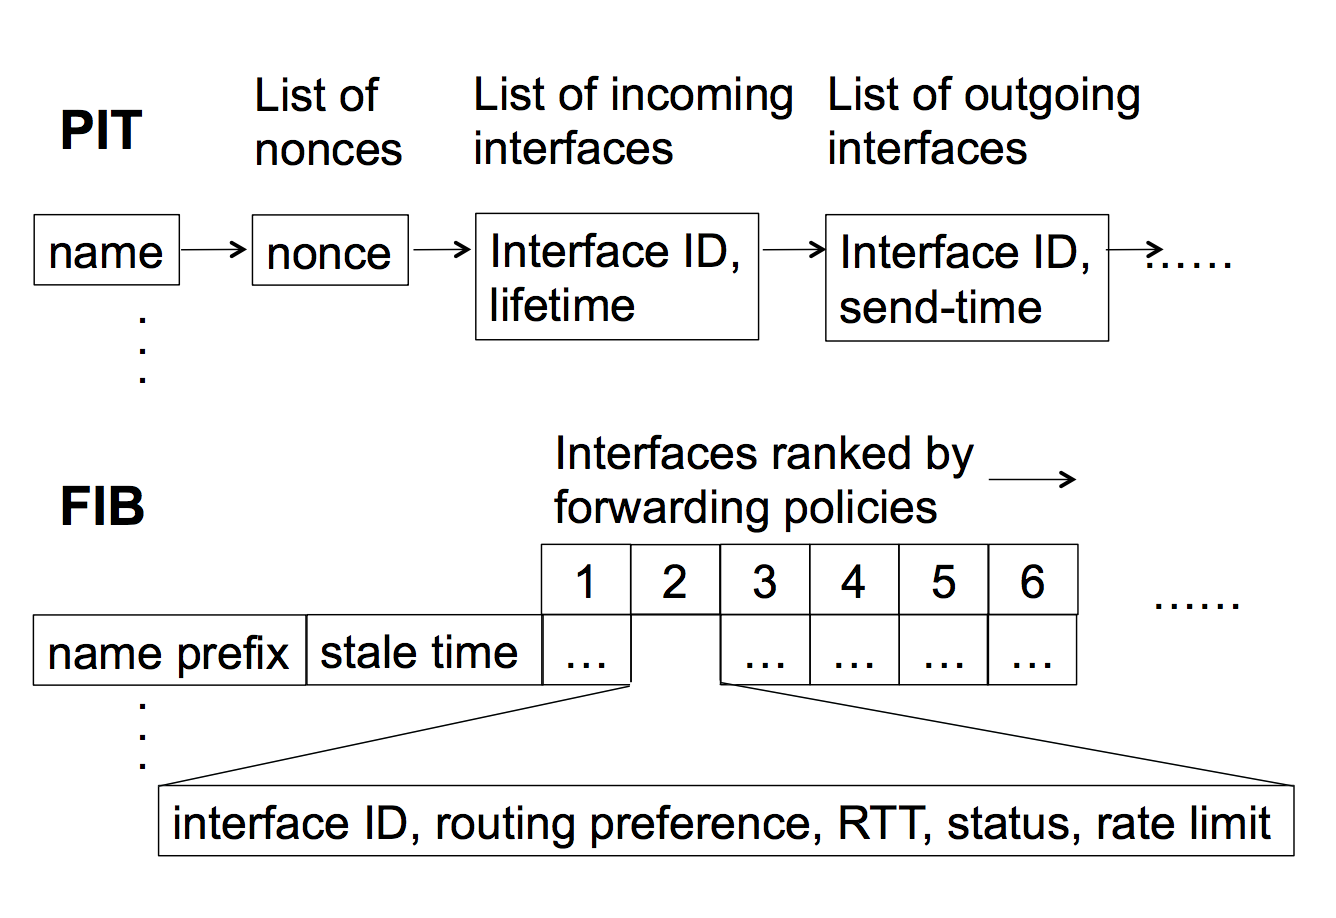
\includegraphics[width=4.5in]{png/pit_fib.png}
\caption{PIT和FIB的结构}
\label{mobility_pic}
\end{figure}

\begin{figure}
\centering
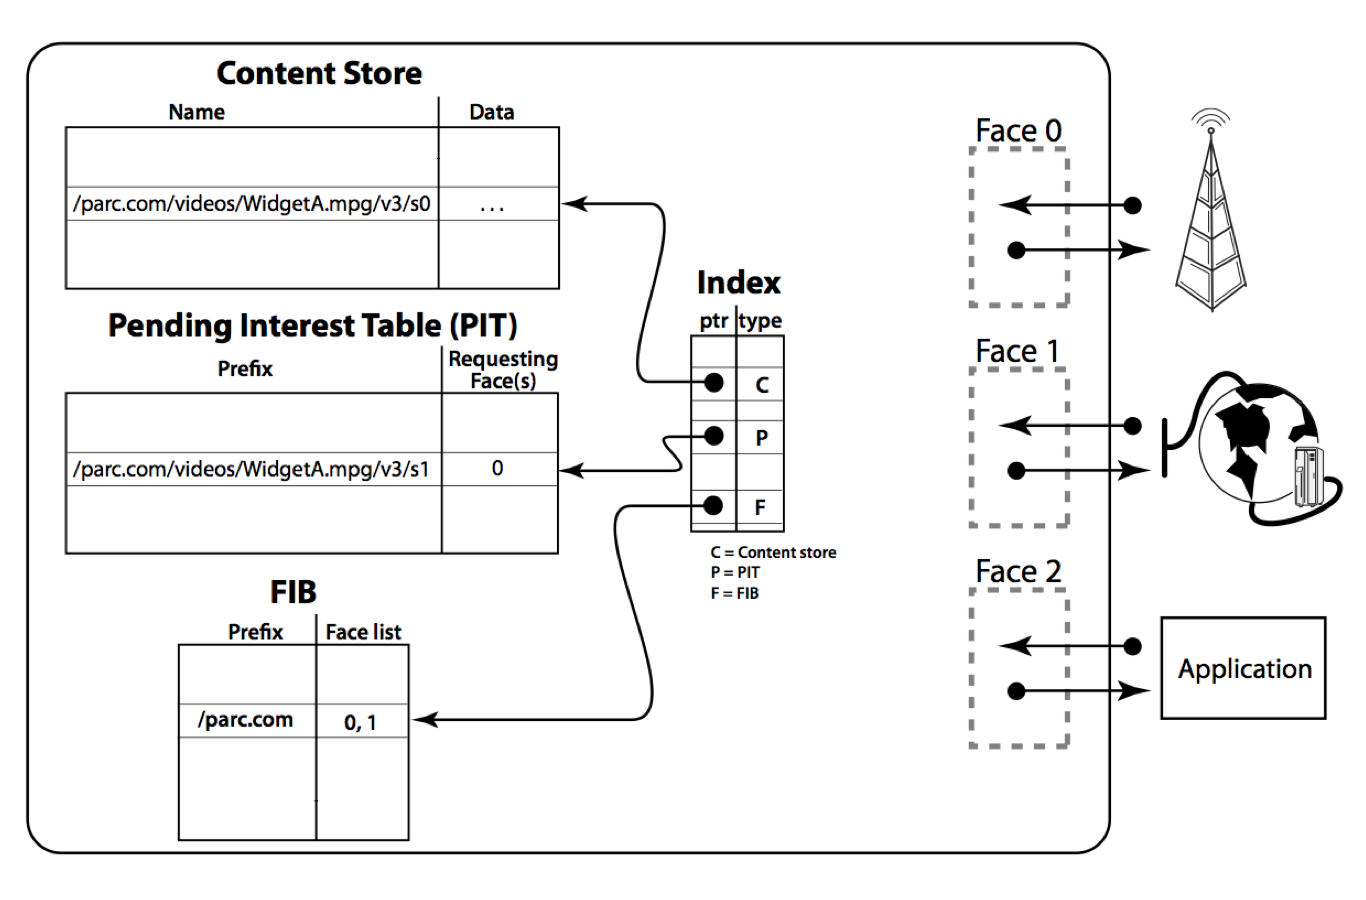
\includegraphics[width=4.5in]{png/forwarding.png}
\caption{一个NDN节点对数据包的转发过程}
\label{mobility_pic}
\end{figure}


一个数据满足一个兴趣包,在每个跃点,实现逐跳流量平衡。
一个NDN数据包与其是来自何处,或在有可能被转发到的位置是独立的,
因此,路由器可以缓存它来满足未来的潜在需求。
这使NDN自动支持各种功能,而无需额外的基础设施,
包括内容分发(许多用户要求在不同的时间相同的数据),
多播(许多用户请求相同的数据在同一时间),
流动性(用户请求来自不同位置的数据),
并延迟容忍网络(用户有间歇连接)。
例如,考虑一个消费者在移动的车辆中观看流媒体视频。
消费者可以请求一些数据,但然后移动到一个新的本地网络。
虽然数据将在到达旧的位置和被丢弃,但是沿着路径会被缓存。
当消费者重发兴趣包,它可能会从附近的一个缓存中提取数据,使得中断最小。
数据缓存接近消费者提高网络传输性能,并减少对特定数据源的依赖。
这样就能有效避免由于故障或攻击可能导致的失败。
